\section{Class Diagrams}

%	Sottolineare il target di tecnologie per cui è effettuata la progettazione. Queste non verranno citate all'interno del capitolo
%	di Progetto ma, il seguente capitolo di Realizzazione, introducendo banalmente le tecnologie utilizzate, dovrà poter
%	calzare perfettamente e dovrà facilmente potersi riallacciare a quanto detto in questo capitolo.

%	In questa sezione si ripercorrono gli stessi argomenti della parte di analisi, in parallelo, ma focalizzandosi sulle scelte di
%	progetto. Queste dovranno essere motivate e lo scopo di questa porzione di testo è di definire le varie parti e la loro 
%	collaborazione GLOBALE (API + persistenza). Il livello di dettaglio non sarà massimo in quanto nelle successive sezioni 
%	si entrerà nello specifico.
%
%	{Diagrammi} Class diagrams UML o analoghi più efficaci per il comportamento dinamico
%	{Immagini}

\section{API}

%	{Analisi prettamente tecnologica}
%	
%	Qui, sulla base di quanto detto nella sezione di analisi, si inizia a mettere insieme le varie parti per descrivere più
%	nel dettaglio l'API dal punto di vista progettuale. Già nella prima parte di analisi è stato introdotto a grandi linee il funzionamento.
%	
%	Il focus è sulle scelte progettuali. Evidenziare dunque i punti di forza e le scelte a livello di pattern.

	Nei successivi paragrafi si spiegherà più nel dettaglio ogni parte attiva all'interno del progetto di queste API, illustrandone e motivandone tutte le scelte progettuali rilevanti.
	Come già deducibile dalla precedente sezione, le API consistono fondamentalmente di due interfacce, \textit{stabili}, \textit{comuni} e \textit{unificate}, che forniscono \textit{Protected Variation} rispetto a rivisitazioni e ottimizzazioni. Pertanto è stato fornito  all'utilizzatore un punto di contatto singolo, una \textit{Facade}, con le librerie.
	
	
	\subsection{Interfaccia ADS}
	
	%	MODELLO FUNZIONALE, motivare la necessità
	%
	%	Sezione in cui si motiva pattern per interfaccia e si evidenzia collegamento funzionale con casi d'uso e requisiti, in termini solo di funzionalità offerte
	
		L'interfaccia dell'ADS, è stata resa parametrica rispetto a tre valori:
		
		\begin{itemize}
			\item \textbf{H}: il tipo dei vari \textit{hash} presenti all'interno dei nodi della struttura.
			\item \textbf{K}: il tipo delle \textit{chiavi} dei nodi.
			\item \textbf{V}: il tipo dei valori presenti nello \textit{storage}. 
		\end{itemize}
	
		Questa scelta rende l'interfaccia applicabile parametricamente rispetto alla scelta dei suddetti tipi, caratteristica utile per garantire flessibilità. 

		Le operazioni fornite dall'ADS, sulla base di requisiti e casi d'uso già discussi in fase di analisi, sono:
		\begin{itemize}
			\item \textbf{\textit{getWithProof(k: K): Pair<V?\footnote{Il punto interrogativo accanto ad un parametro sta ad indicare che quel parametro può essere anche nullo}, Proof<H, K, V>>}}: restituisce il valore $ v $ associato alla chiave $ k $, assieme alla \textit{Proof} per quella chiave. Questa operazione è necessaria per permettere di ottenere la Proof relativa ad una specifica coppia chiave-valore $ (k,v) $.
			\item\textbf{ \textit{getProof(keys: List<K>): Proof<H, K, V>}}: restituisce la Proof relativa alle chiavi contenute nella lista \textit{keys}. Estende le possibilità di \textit{getWithProof(k)}, restituendo in un solo round una Proof cumulativa per un'insieme di chiavi $ keys $, valida e utilizzabile per tutte le stesse. 
			\item \textbf{\textit{getValue(k: K): V?}}: data una chiave $ k $, restituisce il valore $ v $ associato ad essa. Questa operazione permette dunque le operazioni di lettura, \textit{read(k)}, richieste dai casi d'uso.
			\item \textbf{\textit{add(k: K, v: V): H}}: crea un \textit{delta} rispetto alla struttura corrente, il quale viene memorizzato. Il delta riguarda l'aggiunta o la modifica degli elementi relativi alla chiave $ k $. L'operazione \underline{non} modifica la struttura corrente.
			\item \textbf{\textit{del(k: K): H}}: crea un \textit{delta} rispetto alla struttura corrente, il quale viene memorizzato. Il delta riguarda la cancellazione degli elementi relativi alla chiave $ k $ L'operazione \underline{non} modifica la struttura corrente.
			\item \textit{applyDeltas(): ADS<H, K, V>}: compatta tutti i vari delta relativi alla struttura corrente e li applica in ordine, restituendo una nuova ADS, con le modifiche applicate. Questa operazione permette all'ADS di avere la capacità di aggiornarsi rispetto a richieste di update in arrivo dai client.
			\item \textit{rootHash(): H}: calcola e restituisce il \textit{Root Hash} della struttura corrente. Questa operazione permette di ottenere il \textit{digest} dell'intera struttura, come specificato dai requisiti.
			\item \textit{isEmpty(): Boolean}: Informa se l'ADS è vuoto o meno.
		\end{itemize}
	
		E' necessario sottolineare riguardo alla prima operazione fornita, che, per \textit{Creator}, sara l'ADS stesso a generare una Proof una o più chiavi, proprio in quanto è l'unica entità a conoscere le informazioni per farlo. A seguito della creazione, essa sarà un entità indipendente, in grado di aggiornarsi in parallelo rispetto agli update. I calcoli e le operazioni poi eseguite sulla Proof, sono indipendenti dall'ADS di partenza.
		
		Di fondamentale importanza è il requisito relativo alla possibilità di utilizzo dell'ADS in ambito concorrente. Deve essere possibile, dunque, poter operare operazioni in parallelo sull'ADS, senza che ci siano conflitti dovuti alla concorrenza. Pertanto è stato deciso di applicare un principio tipico del paradigma di programmazione funzionale, secondo cui i valori non vengono trovati cambiando lo stato dell'ADS, ma costruendo nuovi stati a partire dai precedenti. Per questo motivo le operazioni di scrittura, ovvero quelle che modificherebbero lo stato della struttura, lo fanno in maniera totalmente compatibile con quanto detto. Una spiegazione più dettagliata di come questo sia stato realizzato è posticipata in paragrafi successivi.
		
		La scelta invece di disaccoppiare il momento dell'individuazione della operazioni di aggiunta, modifica o cancellazione, dal momento della loro effettiva applicazione, è da inquadrare in un contesto più ampio di utilizzo della libreria. Intuitivamente, questa funzionalità è fornita per permettere di gestire meglio gli stati in cui si può trovare la struttura stessa: ad esempio uno stato in cui può ricevere e accumulare update, piuttosto che uno stato in cui questi vengono applicati in blocco. Migliore è di conseguenza la gestione delle operazioni di lettura, in quanto per garantirne la consistenza, esse possono essere collocate in istanti temporali diversi, prima o dopo determinati stati della struttura.
		
		L'interfaccia, e dunque la classi che implementeranno quest'ultima, deve implementare a sua volta l'interfaccia \textit{Serializable}, in quanto dovrà avere la caratteristica di essere, appunto, serializzabile. Questo è motivato dal fatto che implementazioni di questa interfaccia saranno inserite all'interno di messaggi che dovranno essere spediti su rete, nell'ambito dell'utilizzo di questa API.
	
	\subsection{Interfaccia Proof}
	
	%	MODELLO FUNZIONALE, motivare la necessità
	%
	%	Sezione in cui si motiva pattern per interfaccia e si evidenzia collegamento funzionale con casi d'uso e requisiti, in termini solo di funzionalità offerte
		
		L'interfaccia della Proof, è stata resa parametrica rispetto a tre valori:
		
		\begin{itemize}
			\item \textbf{H}: il tipo dei vari \textit{hash} presenti all'interno dei nodi della Proof.
			\item \textbf{K}: il tipo delle \textit{chiavi} dei nodi.
			\item \textbf{V}: il tipo dei valori presenti nello \textit{storage}. 
		\end{itemize}
		
		Questa scelta rende l'interfaccia applicabile parametricamente rispetto alla scelta dei suddetti tipi, caratteristica utile per garantire flessibilità. 
		
		Le operazioni fornite dalla Proof, sulla base di requisiti e casi d'uso già discussi in fase di analisi, sono:
		\begin{itemize}
			\item \textbf{\textit{keys: Set<K>}}: insieme contenente tutte le chiavi per cui è valida la Proof.
			\item \textbf{\textit{rootHash(): H}}: restituisce il \textit{Root Hash} della Proof. Questa, assieme alla successiva, sono requisiti funzionali già discussi in fase di analisi.
			\item \textbf{\textit{rootHash(list: List<Pair<K, V>>): Proof<H, K, V>}}: applica gli aggiornamenti specificati nella lista di coppie chiave-valore \textit{list} e successivamente calcola e restituisce il nuovo \textit{Root Hash}.
			\item \textbf{\textit{union(proof: Proof<H, K, V>): Proof<H, K, V>}}: effettua il \textit{merge} di due Proof relative allo stesso istante temporale della stessa struttura da cui sono state generate. Restituisce una nuova proof, cumulativa rispetto a quelle di partenza.
		\end{itemize}
		
		Di fondamentale importanza è il requisito relativo alla possibilità di utilizzo della Proof in ambito concorrente. Deve essere possibile, dunque, poter operare operazioni in parallelo sulla Proof, senza che ci siano conflitti dovuti alla concorrenza. Pertanto è stato deciso di applicare un principio tipico del paradigma di programmazione funzionale, secondo cui i valori non vengono trovati cambiando lo stato della Proof stessa, ma costruendo nuovi stati a partire dai precedenti. Per questo motivo le operazioni di scrittura, ovvero quelle che modificherebbero lo stato della struttura, lo fanno in maniera totalmente compatibile con quanto detto. Una spiegazione più dettagliata di come questo sia stato realizzato è posticipata in paragrafi successivi.
		
		L'interfaccia, e dunque la classi che implementeranno quest'ultima, deve implementare a sua volta l'interfaccia \textit{Serializable}, in quanto dovrà avere la caratteristica di essere, appunto, serializzabile. Questo è motivato dal fatto che implementazioni di questa interfaccia saranno inserite all'interno di messaggi che dovranno essere spediti su rete, nell'ambito dell'utilizzo di questa API.
	
	\subsection{Nodo e schema hashing}
	
	%	Parlare dell'elemento alla base di implementazioni realizzate di ADS e Proof.
	%
	%	Breve sezione che riprende l'argomento dell'hashing e che lo analizza concentrandosi sulle scelte progettuali. Si parla anche della parametrizzazione rispetto
	%	alle varie funzioni di hashing e si parla di HashUtils con relativo pattern Singleton
	
	L'elemento base costituente sia della Skip List Autenticata sia della Skip List Proof, è il \textit{nodo}. Esso, oltre ad essere a conoscenza dei suoi nodi adiacenti, nelle quattro direzioni, \textit{next}, \textit{prev},  \textit{up} e \textit{down}, è formato da tre campi interni:
	\begin{itemize}
		\item \textbf{Key}: Un attributo chiave necessario per la struttura in cui è collocato a mantenere l'ordinamento. Il tipo $ K $ della chiave \underline{deve} dunque necessariamente implementare l'interfaccia \textit{Comparable<K>}.
		\item \textbf{First Hash}: Un campo che contiene l'hash relativo al nodo immediatamente inferiore , \textit{down} ,o l'hash del valore dello storage relativo a questo nodo.
		\item \textbf{Second Hash}: Un campo che contiene l'hash relativo al nodo successivo,  \textit{next}, se quest'ultimo è presente.
	\end{itemize}

	La scelta di tripartire all'interno del nodo le sezioni sopra menzionate, è stata presa sia per poter rispettare nella maniera più comoda e flessibile lo schema di hashing già discusso in fase di analisi, e sia per ridurre la quantità di operazioni per il refresh di tutta la struttura, a seguito di operazioni di update. Infatti a seguito di una operazione di inserimento, modifica o cancellazione, sarà necessario aggiornare solamente i campi strettamente interessati.
	
	Il campo \textit{down}, si precisa, che può essere sia una nodo, nella maggior parte dei casi, ma anche il valore vero e proprio, presente nello storage classico, legato a questo nodo. Sarà dunque solo ed esclusivamente questo nodo a conoscere questo valore e a memorizzare il suo hash nel campo \textit{first Hash}.
	
	La classe che implementa il nodo, deve implementare l'interfaccia \textit{Serializable}, in quanto dovrà avere la caratteristica di essere, appunto, serializzabile. Questo è motivato dall'inserimento di oggetti di questo tipo all'interno di messaggi che dovranno essere spediti su rete, nell'ambito dell'utilizzo di questa API.
	
	Lo schema di hashing presente all'interno della struttura, rispecchia quello già presentato in fase di analisi, e si adatta perfettamente alla separazione dei valori di hash attuata all'interno del nodo. Infatti da un lato il campo \textit{first Hash}, memorizzerà sempre l'hash relativo al campo \textit{down} del nodo, sia esso un nodo o un valore vero e proprio, di tipo qualsiasi. Dall'altro lato il campo \textit{second Hash} memorizzerà, solo se presente, l'hash relativo al campo \textit{next} del nodo corrente. 
	E' stato ritenuto conveniente eliminare, per i nodi sulla \textit{base list}, il fatto che il campo \textit{second Hash}, nel caso in cui il nodo \textit{next} sia un nodo \textit{tower}, dovesse memorizzare l'hash relativo al valore sottostante il nodo \textit{next}. Questo permette di garantire l'esecuzione di tutte le operazione che comportino un refresh degli hash della struttura, in un tempo che sia con alta probabilità, $\mathcal{O}(log{}n)$.
	Inoltre, la proprietà di non-commutatività degli hash, si manifesta nel fatto che, per costruzione, se fosse invertito il valore presente nel campo \textit{first Hash}, con quello presente nel campo \textit{second Hash}, il cambiamento si ripercuoterebbe su tutti gli hash seguenti, fino ad arrivare alla modifica del root Hash dell'intera struttura. Pertanto è fondamentale l'ordine e la posizione reciproca dei vari nodi.
	
	Per quanto riguarda più specificatamente le funzioni crittografiche di hash, si è deciso di delegare il compito di calcolo di hash, singoli o concatenati, ad un \textit{Singleton}, visibile a tutte le classi dell'API. Questa scelta ha permesso di rendere l'intera realizzazione totalmente flessibile e parametrica rispetto alla particolare funzione di hash che si volesse adottare, tra quelle disponibili elencate in fase di analisi.
	
	\begin{figure}
		\centering
		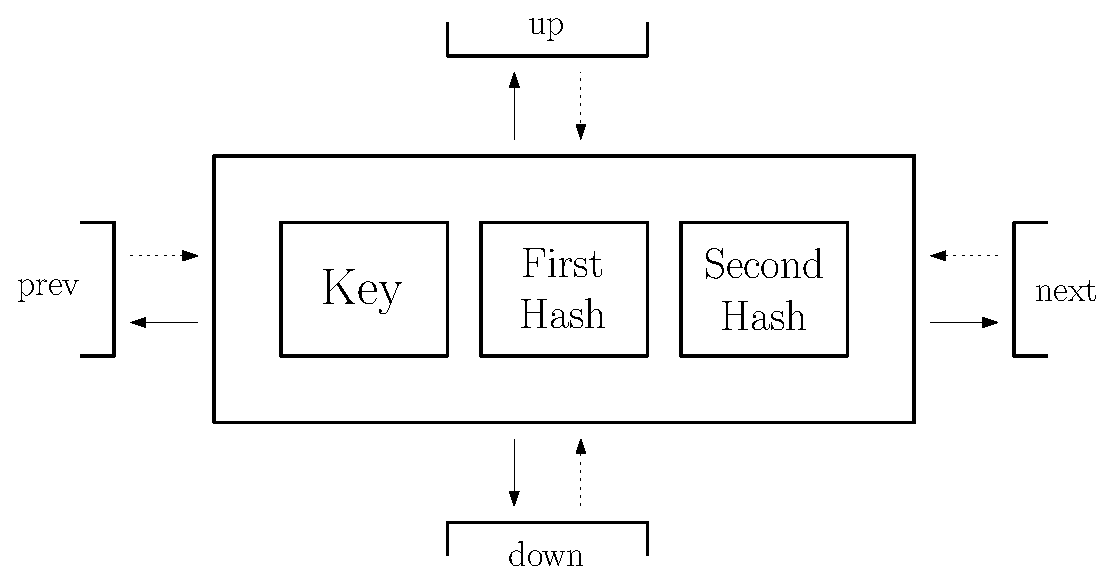
\includegraphics[scale=0.6]{figure/nodo.eps}
		\caption{Esempio di un nodo.}\label{fig:1}
	\end{figure}
		
	\subsection{Skip List Autenticata}
	
	%	MODELLO FUNZIONALE, motivare la realizzazione
	%	
	% 	Fatte tutte le opportune premesse descritte e motivate (APS style), si passa ora alla descrizione della struttura principale
	
	Prima di addentrarsi dettagliatamente su aspetti di natura progettuale e algoritmica della struttura dati autenticata, è necessario fare delle considerazioni di carattere generale, conseguenza di quanto detto in fase di analisi.
	Prima di tutto si sottolinea l'inutilità, in questo studio progettuale, della colonna di nodi sentinella di tipo $ +\infty $, la cui presenza comporterebbe solo un inutile spreco di memoria. I nodi sentinella di tipo $ -\infty $, d'altro canto, servono sia per poter avere una colonna che sia concettualmente antecedente a tutte le altre colonne presenti nella struttura e sia di supporto all'applicazione dello schema di hashing.
	Secondariamente si è ritenuto superfluo, e puramente formale, il mantenimento di un livello superiore a tutti gli altri livelli, contenente soltanto agli estremi i nodi sentinella. Questo aggiungerebbe solamente una passo in più agli algoritmi di esecuzione delle operazioni. Nel contesto più ampio di una successiva applicazione di memorizzazione in persistenza della struttura, il mantenimento di questo livello superiore complicherebbe soltanto la conversione da formato ad oggetti a quello della base di dati.
	
	La ricerca in tempo logaritmico, cosi come le operazioni di inserimento, cancellazione o modifica, sono permesse dalle chiavi dei nodi, che dunque saranno ordinate: $ k_{-\infty} < k_{1} < k_{2} < \dots < k_{n} < k_{+\infty} $.
	
	\begin{figure}[tbp] 
		\begin{center}
			\begin{tabular}{c @{\hspace{1em}} c}
				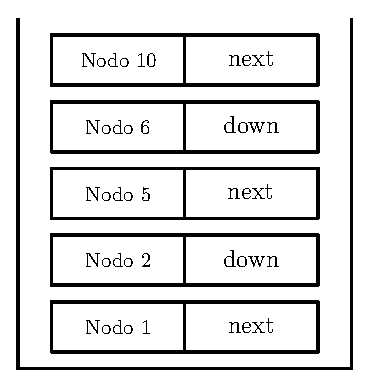
\includegraphics[scale=0.7]{figure/stack.eps} &
				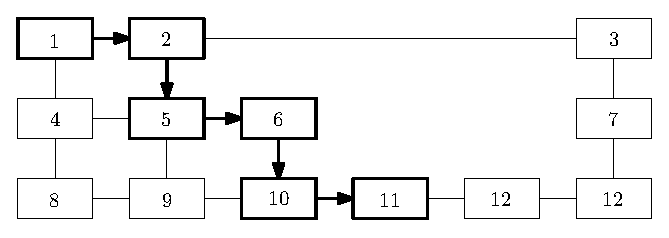
\includegraphics[scale=0.6]{figure/path.eps} \\
				(a) & (b)
			\end{tabular}
		\end{center}
		\caption{Esempio di una pila. I nodi sono stati volutamente segnati con un identificativo, per facilitare la comprensione dell'immagine, ma non hanno alcun riferimento con la progettazione o la realizzazione reale dei nodi. (a) La pila contenente in ordine di attraversamento, dal basso verso l'alto, i passi compiuti per comporre il \textit{path}. I blocchi della pila sono composti dal nodo di partenza di ogni passo, affiancato dalla stringa che indica la direzione del passo compiuto. (b) Sono evidenziati, nella Skip List, i nodi e le direzioni presenti nello stack, a seguito della ricerca dell'elemento 10.} \label{fig:stack+path}
	\end{figure}
	
	Segue la descrizione delle operazioni fornite, con enfasi sulle caratteristiche algoritmiche:
	
	\begin{itemize}
		\item \verb!getWithProof(k: K): Pair<V?, Proof<H, K, V>>!. L'algoritmo alla base di questa funzione, può essere diviso in due parti. La prima parte effettua una semplice ricerca di $ k $ sulla base delle chiavi contenute nei nodi, costruendo contemporaneamente la pila, \textit{stack}, di cui un esempio è raffigurato in figura \ref{fig:stack+path}. Questa funzione, come tutte le operazioni di read offerte dalla Skip List Autenticata, si appoggiano su una serie di metodi per la ricerca, che oltre a restituire il nodo cercato, riempono la pila con opportuni dati per ogni passo effettutato. La seconda parte sfrutta proprio il contenuto di questa pila, per poter costruire la \textit{Proof} relativa alla chiave cercata $ k $. Infatti il contenuto della pila, analizzato a ritroso rispetto all'ordine di riempimento, rappresenta il percorso, \textit{path}, inverso, dal nodo allo \textit{start node.}. Per costruire la Proof necessaria ad ottenere il \textit{root hash}, bisogna però "integrare" i nodi presenti nello stack, proprio per costruzione dello schema di hash adottato sulla struttura. Se, ad esempio, un nodo ha come \textit{next} un \textit{plateau}, allora esso dovrà essere inserito nella \textit{Proof} in quanto sarà necessario nella computazione degli hash. Lo stesso vale per i nodi \textit{down} di ogni nodo, che non siano presenti già nel \textit{path}.
		In base a quanto detto, una volta effettuata la ricerca dell'elemento, che indirettamente costituisce la pila, viene ripercorso il \textit{path} a ritroso partendo dall'elemento trovato, con opportune operazioni di pop. Ogni operazione di pop fornisce il successivo nodo presente nel \textit{path} e la direzione, in senso inverso, che deve essere intrapresa per raggiungerlo. Tramite questa seconda informazione è possibile distinguere il caso in cui, seguendo il \textit{path}, è necessario proseguire verso sinistra o verso l'alto. Nel primo caso sarà necessario integrare la \textit{Proof} con il nodo \textit{down} del successivo nodo del \textit{path}. Nel secondo caso, invece l'integrazione avviene solo nel caso in cui il nodo \textit{next} del successivo nodo del \textit{path} sia un \textit{plateau}.
		
		\item \verb!getProof(keys: List<K>): Proof<H, K, V>!. Questa funzione in qualche modo estende la precedente, dando la possibilità, in un solo round, di richiedere ed ottenere una Proof valida per un insieme di chiavi passato come parametro. Ovviamente la lista passata dovrà necessariamente contenere solo chiavi presenti nella struttura.
		Per raggiungere questo obiettivo, da un lato la struttura si preoccupa di creare le singole Proof, una per volta, per ogni singola chiave passata come parametro, in quanto, come già detto, è l'unica entità che conosce le informazioni necessarie a farlo. Dall'altro è mantenuta una Proof cumulativa, valida per tutte le chiavi nell'intervallo $ [k[0], k[corrente]] $. Pertanto appena è creata una nuova Proof viene integrata con la Proof cumulativa corrente, richiedendo a quest'ultima una \verb!union(proof: Proof<H, K, V>)!. Questo procedimento prosegue fino all'avvenuta presa in considerazione dell'ultima chiave in $ keys $, e termina con la restituzione della Proof cumulativa, a questo punta valida per tutto l'insieme di chiavi passato per parametro.
		
		E' inoltre necessario precisare che la Skip List Autenticata risulta accoppiata all'interfaccia della Proof, e \textit{non} alla sua implementazione. Questo è stato preferito, fornendo uno strato di \textit{Indirection}, in quanto la Skip List Proof, può subire cambiamenti e ottimizzazioni interne, senza ripercuotersi direttamente sulla Skip List Autenticata.
		
		\item \verb!getValue(k: K): V?!. Si tratta di una semplice operazione di \textit{retrieve}. Infatti restituisce un valore di tipo $ V $, associato alla chiave $ k $ passata come parametro. Se non è presente la chiave è restituito $ null $.
		
		\item \verb!applyDeltas(): ADS<H, K, V>!. Questa operazione permette alla struttura di avere la capacità di aggiornarsi rispetto a richieste di update in arrivo dai client. Trattandosi di una operazione di scrittura, e dovendo innestarsi in un ambito di concorrenza già altrove menzionato, sarà necessario evitare di modificare direttamente lo stato della struttura. Dunque viene separato il momento della ricezione di particolari richieste di update dal momento della loro effettiva applicazione. In questo modo sarà possibile \textit{clonare} la struttura corrente e applicare su quest'ultima gli update. Gli update possono tradursi in primitive di tipo \verb!add(k: K, v: V): H! nel caso si trattasse di aggiunte o modifiche, o di tipo \verb!del(k: K): H! nel caso si trattasse di cancellazioni, andando rappresentare dei \textit{delta}, ossia delle variazioni in potenza della struttura. Essi sono accumulati, mantenendone l'ordine di "arrivo" in una pila, con opportune operazioni di $ push $. A seguito dell'invocazione di \verb!applyDeltas()!, le istanze della pila vengono valutata una ad una singolarmente, in ordine cronologico, con operazioni di $ pop $, e applicate a un clone della struttura corrente. Sarà poi questo, comprensivo degli update, ad essere restituito.
		L'attuazione effettiva delle varie azioni presenti all'interno della pila, è scissa, con l'obiettivo di migliorare la coesione generale, tra l'operazione \verb!applyAdd(k: K, v: V)! nel caso di aggiunte o modifiche, e l'operazione di \verb!applyDel(k: K)! nel caso di cancellazioni.
		Queste scelte rendono invariato lo stato della struttura di partenza, che sarà dunque passibile di calcoli e computazioni anche contemporaneamente all'applicazione di update.
					
		\item \verb!rootHash(): H!. Operazione che calcola e restituisce il \textit{Root Hash} dell'intera struttura. Lo \textit{Start node} conterrà in ogni istante, nel campo \textit{firstHash}, il contributo in termini di concatenzioni di hash crittografici dato da tutti gli elementi correlati al campo \textit{down}, e nel campo \textit{secondHash}, il contributo in termini di concatenazioni di hash crittografici dato da tutti gli elementi correlati al campo \textit{next}. Viene, a questo punto, restituito l'hash derivato dalla concatenazione dei campi \textit{firstHash} e \textit{secondHash}.
			
		\item \verb!isEmpty(): Boolean!. Questa operazione semplicemente restituisce \textit{true} se la struttura non contiene nessuna coppia chiave-valore, \textit{false} altrimenti.

%	  [Appunti di ragionamento su cloning ADS]		
		\item \verb!clone(): ADS<H, K, V>!. Copia la struttura e ne restituisce una identica, tranne per i delta che \underline{non} vengono copiati. Il problema della clonazione è di non banale risoluzione. Infatti la Skip List Autenticata è a tutti gli effetti un grafo diretto ciclico. Una prima possibilità potrebbe consistere nel clonare ogni torre iterando sulla \textit{base list}, per poi preoccuparsi solo in un secondo momento dei collegamenti orizzontali. La struttura della Skip List però comporterebbe una scansione di tutte queste torri clonate per ogni nodo di ogni torre, operazione con costo computazionale molto elevato e non auspicabile. Richiederebbe inoltre la conoscenza, diretta o indiretta, dell'altezza di ogni singola torre. 
		Per motivi analoghi, è da escludere anche la soluzione simmetrica, che memorizza ogni livello orizzontale, per poi preoccuparsi solo in un secondo momento dei collegamenti verticali.
		La soluzione poi effettivamente adottata, consiste nell'utilizzo di \textit{Hash Map} di supporto, una per ogni livello della Skip List Autenticata, tutte di lunghezza pari alla dimensione della \textit{base list} della struttura e tutte contenenti \textit{entries} con tutte le chiavi della struttura. Iterando orizzontalmente su ogni livello, le Hash Map corrispondenti saranno riempite. A seconda del nodo scansionato, verrà aggiunto un riferimento a quest'ultimo nella \textit{entry} corrispondente nella Hash Map. Se per una determinata chiave non sarà presente il nodo corrispondente a quel determinato livello, verrà mantenuto il valore di quella \textit{entry} a null. Così facendo sarà possibile avere tutti i riferimenti ad ogni nodo, e allo stesso tempo conoscerne l'esatta collocazione reciproca. Sarà possibile poi clonare ogni singolo nodo, e sostituire il riferimento contenuto nei vari valori delle Hash Map con i vari cloni. A questo punto sarà necessario solo provvedere ai collegamenti, sia orizzontali che verticali. Per quanto riguarda i collegamenti verticali sarà sufficiente collegare tutti i nodi con stessa chiave su Hash Map corrispondenti a livelli adiacenti. Per quanto riguarda i collegamenti orizzontali sarà necessario collegare i nodi adiacenti all'interno di una stessa Hash Map, intervallati cioè da sole \textit{entries} con valori nulli.	
		
	\end{itemize}

%	\begin{figure}
%		\centering
%		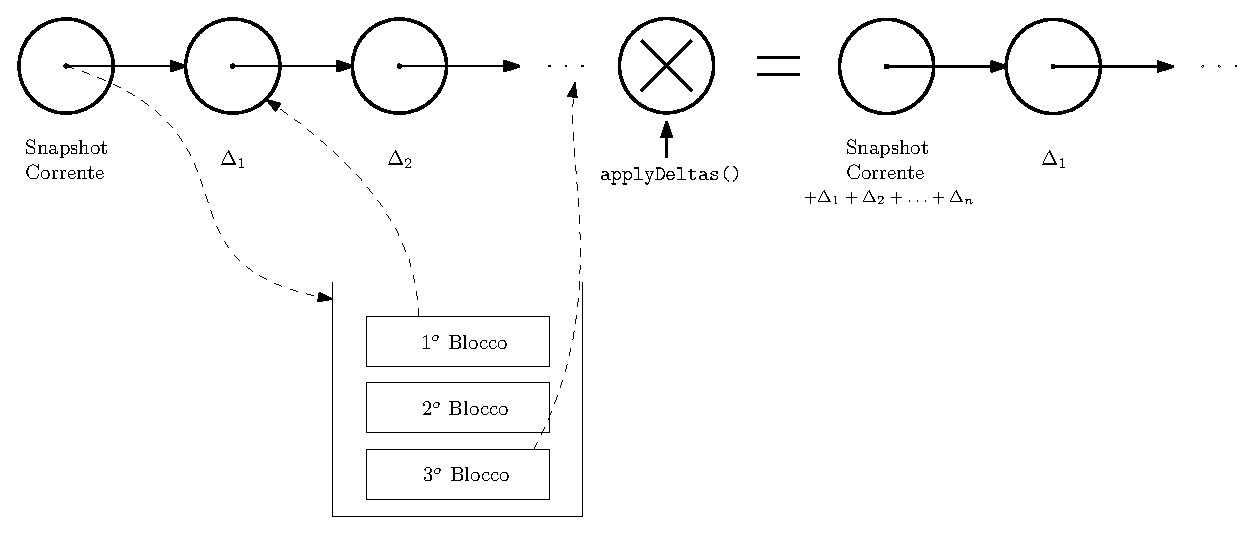
\includegraphics[scale=0.6]{figure/deltas.eps}
%		\caption{Schema che mostra il funzionamento dei \textit{delta}. Tramite primitive di tipo \verb!add(k: K, v: V)! e/o \verb!del(k: K)! si popola la pila della struttura con dei blocchi, ordinati cronologicamente. L'uso di \verb!applyDeltas()! applica in ordine questi \textit{delta} e restituisce un'altra struttura, con stato di partenza equivalente al primo \textit{snapshot}, ma con tutti i $\Delta_{n}$ applicati. La pila viene svuotata, ed è dunque poi pronta ad accogliere nuovi \textit{delta}.}\label{fig:delta}
%	\end{figure}

	\begin{figure}
		\centering
		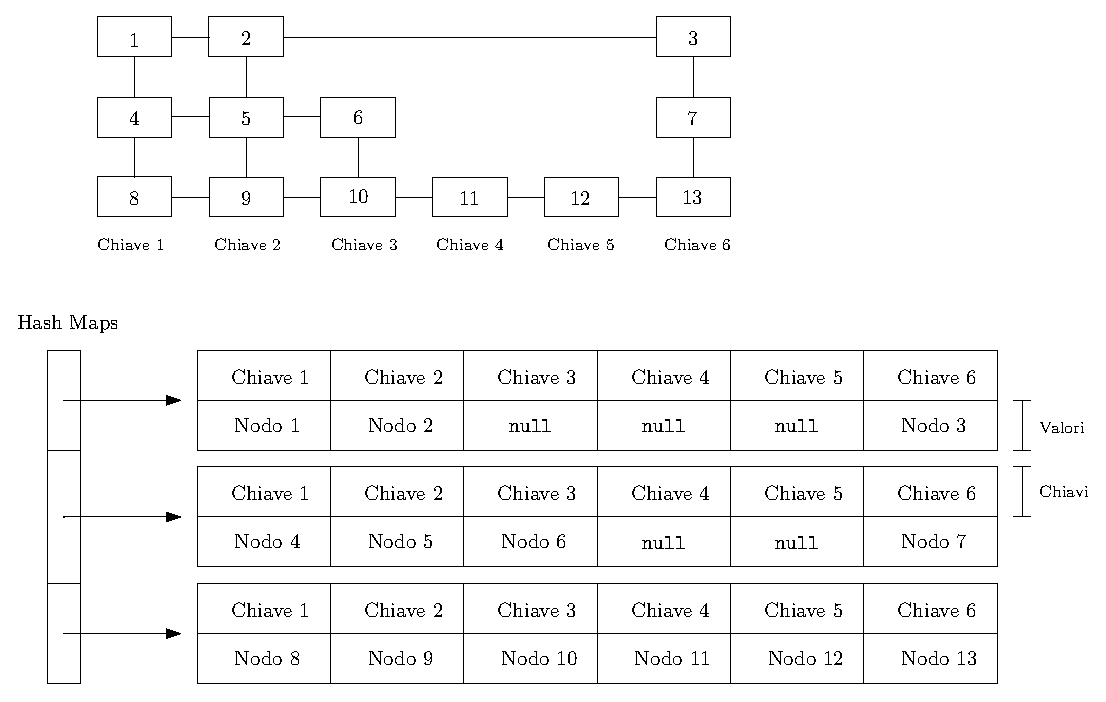
\includegraphics[scale=0.6]{figure/cloneADS.eps}
		\caption{Immagine che illustra un esempio di Hash Map, come sarebbero nella prima fase dell'operazione di clonazione, rispetto alla Skip List nell'esempio. E' possibile poi da questo stato clonare tutti i nodi e provvedere alla sistemazione di tutti i collegamenti.}\label{fig:cloneADS}
	\end{figure}
	
	\subsection{Skip List Proof}
	
	%	MODELLO FUNZIONALE, motivare la realizzazione
	%	
	%	Fatte tutte le opportune premesse descritte e motivate (APS style), si passa ora alla descrizione della struttura skip list proof
	

		Prima di addentrarsi dettagliatamente su aspetti di natura progettuale e algoritmica della Skip List Proof, è necessario fare delle premesse. La Proof, come già detto, concettualmente parlando, è relativa ad un particolare istante temporale della struttura dati autenticata da cui è stata generata. Dunque dal momento in cui inizia ad esistere, acquisisce uno stato e questo sarà completamente indipendente dallo stato della struttura di partenza. Pertanto la Skip List Proof, sarà una struttura dati indipendente e parallela all'ADS di partenza, di cui, inoltre, non avrà nessuna conoscenza, per motivi in parte già comprensibili, e in parte motivati in seguito nella sezione dedicata alla persistenza.

		In base all'utilizzo dell'API, inoltre, nell'ambito del protocollo di integrità su dati nel Cloud (6), sarà necessario poter applicare update ricevuti dall'ADS, nella forma compatibile con la Proof, alla Proof stessa, come già detto indipendente dalla struttura da cui è stata generata.
		
%	  [Discorso su somiglianza con albero]
		Fatti questi ragionamenti di natura concettuale, ora si riporta il ragionamento alla base di alcune decisioni progettuali e algoritmiche. La Proof per una chiave , rispetto alla Skip List Autenticata da cui è generata, è a tutti gli effetti poco più di un percorso, \textit{path}, dal nodo contenente quella specifica chiave, fino allo \textit{start node}. Gli elementi che ha in più sono i nodi necessari a ricostruire tutto il percorso di concatenazioni di hash necessarie a calcolare e restituire il \textit{Root Hash}, e sono o $ plateau $ presenti nel campo $ next $ di un nodo, non già presenti nel path, o nodi presenti nel campo $ down $ di un nodo, non già presenti nel path. La Proof cumulativa rispetto a un insieme di chiavi non fa altro che estendere la struttura corrente con ulteriori "path".
		Si potrebbe dunque pensare di rappresentare la Proof come fosse un albero binario, dove per ogni nodo, al posto di avere figlio destro e sinistro, si hanno rispettivamente nodo $ next $ e nodo $ down $. Tuttavia è facile dimostrare che la struttura sarebbe fortemente sbilanciata e risulterebbe oneroso computazionalmente, tra le varie foglie che si verrebbero a formare, trovare quali sono le chiavi per cui la Proof è valida, a meno che non si utilizzi una struttura dati di supporto per memorizzare i riferimenti a tali nodi. Rimarrebbe tuttavia non ottimale per quanto riguarda l'applicazione di aggiornamenti alla struttura.
 				
%	  [Discorso per giungere alla somiglianza con skip list] ==> [Motivare il nome del paragrafo e dunque della struttura]
		Si è preferito dunque utilizzare una struttura dati \textit{ad hoc}, con forti somiglianze con la Skip List Autenticata. I nodi e l'organizzazione interna saranno dunque uguali alla controparte. Le differenze principali risiedono nell'utilizzo di molti meno puntatori inter-nodo e nell'assenza di qualsiasi riferimento ai valori dello storage classico, prerogativa esclusiva dell'ADS. I nodi corrispondenti alla \textit{base list} avranno conoscenza solo dell'hash di questi valori.
		In questo modo inoltre, molte delle proprietà caratteristiche della Skip List, sarebbero ereditate da questa struttura, chiamata per ovvi motivi, \textit{Skip List Proof}, da cui il titolo del paragrafo.
		
%     [Discorso su scelta tra opzione HEAD e opzione KEYS]  ==> [Menzionare che lo start node è lo stesso della skip list autenticata]
		Riguardo la gestione interna della struttura, si individuano due principali alternative. La prima consiste nell'utilizzare come punto di partenza per ogni operazione il nodo \textit{HEAD}, corrispondente allo \textit{start node} della Skip List Autenticata. La seconda invece consiste nell'avere una struttura contenente i riferimenti ai nodi contenenti le coppie chiave-valore per le quali è valida la Proof. La seconda soluzione presenta dei vantaggi soprattutto per quanto riguarda le operazioni che devono essere effettuate su un specifiche chiavi, in quanto sarebbe possibile sostituire l'operazione di ricerca vera e propria, con un veloce accesso indicizzato. Tuttavia, come soluzione, risulterebbe svantaggiosa per tutti i calcoli che riguarderebbero il nodo \textit{HEAD}, in quanto non sarebbe presente un riferimento fisso a quest'ultimo. La soluzione poi realmente adottata è un ibrido tra le due. Sarà dunque utilizzato il riferimento al nodo \textit{HEAD} per le operazioni \verb!rootHash(): H! e \verb!union(proof: Proof<H, K, V>): Proof<H, K, V>! e la struttura proposta nella seconda soluzione, per ridurre di un fattore $\mathcal{O}(m)$ la complessità computazionale dell'operazione \verb!rootHash(list: List<Pair<K, V?>>): Pair<Proof<H, K, V>, H>!, la quale nel caso di adozione esclusiva della prima soluzione sarebbe dell'ordine di $\mathcal{O}(m^{2}*n)$, dove $ m $ è il numero di nodi nel \textit{path} di ogni singola Proof, e $ n $ è il numero di chiavi per cui è valida la Proof stessa.
		
						
		Segue la descrizione delle operazioni fornite, con enfasi sulle caratteristiche algoritmiche:
		
		\begin{itemize}
%			\item \verb|findNode(key: K, start: AuthSkipListNode<K, H>? = null): AuthSkipListNode<K, H>|. E' un operazione di ricerca. Intuitivamente, per costruzione di Skip List Proof, è analoga ai metodi di ricerca all'interno della Skip List Autenticata. Partendo dall'\textit{HEAD} o dal nodo $ start $ se passato per parametro, in base alla chiave $ key $ è effettuata la ricerca del nodo corrispondente. Se la chiave inserita non è presenta è necessario sia sollevata un'eccezione, altrimenti viene restituito il nodo trovato. Questa operazione è privata e di supporto alle successive operazioni, nel caso di sola adozione della soluzione con nodo \textit{HEAD}.
			
			\item \verb!rootHash(): H!. L'operazione è analoga a quella della Skip List Autenticata appena descritta. Calcola e restituisce il \textit{Root Hash} dell'intera proof. Il nodo \textit{HEAD} conterrà in ogni istante, nel campo \textit{firstHash}, il contributo in termini di concatenzioni di hash crittografici dato da tutti gli elementi correlati al campo \textit{down}, e nel campo \textit{secondHash}, il contributo in termini di concatenazioni di hash crittografici dato da tutti gli elementi correlati al campo \textit{next}. Viene, a questo punto, restituito l'hash derivato dalla concatenazione dei campi \textit{firstHash} e \textit{secondHash}.
			
			\item \verb!rootHash(list: List<Pair<K, V?>>): Pair<Proof<H, K, V>, H>!. Nel caso in cui tutti i valori passati siano nulli, l'operazione risulta equivalente a \verb|rootHash(): H|. Tramite la presenza di anche un solo valore non nullo, l'operazione diventerà di scrittura. Trattandosi di una operazione di scrittura, e dovendo innestarsi in un ambito di concorrenza già altrove menzionato, sarà necessario evitare di modificare direttamente lo stato della struttura. Dunque la struttura sarà clonata internamente e le modifiche agli hash saranno applicate sul clone. La struttura iniziale sarà dunque passibile di calcoli e computazioni anche contemporaneamente all'applicazione di queste modifiche. Il parametro che accetta è una lista di coppie chiave-valore, struttura che verrà processata iterativamente, rendendo superflua l'applicazione di una mappa di coppia chiave-valore. Nello specifico l'operazione processerà, per ogni chiave presente nella lista $ list $, il nodo corrispondente nella Proof, aggiornando gli hash, risalendo fino al nodo \textit{HEAD}. Al termine di questo elenco di queste operazioni, la funzione restituirà la nuova Proof, con le modifiche applicate e il nuovo \textit{Root Hash}.
			
			\item \verb!union(proof: Proof<H, K, V>): Proof<H, K, V>!. Trattandosi di una operazione di scrittura, e dovendo innestarsi in un ambito di concorrenza già altrove menzionato, sarà necessario evitare di modificare direttamente lo stato della struttura. Dunque la struttura sarà clonata internamente e l'unione verrà effettuta sul clone. L'unione consiste, intuitivamente, nell'integrazione della Proof su cui viene invocato il metodo, $ this $, con la Proof passata per parametro, $ proof $. Inizia, infatti, col trovare, tramite differenza tra insiemi, le chiavi presenti in $ proof $ che non sono presenti in $ this $. Per ognuna di queste chiavi risultato della differenza, se presenti, viene effettuata una iterazione parallela a partire dall'HEAD di $ this $ e dall'HEAD di $ proof $. che ha come fine quello di aggiungere a $ this $ i nodi per renderla valida per le ulteriori chiavi, contributo di $ proof $. E' mostrato in maniera più chiara nel seguente pseudocodice:
		
			\begin{algorithm}[H]
				\ForEach{key in (proof.keys - this.keys)}{
					first-iterator = this.head
					second-iterator = proof.head
					\If{second-iterator.next != null}{
						first-iterator.next = second-iterator.next
					}
					\If{second-iterator.down != null}{
						first-iterator.down = second-iterator.down
					}
					\eIf{second-iterator.next.key $ \leq $ key}{
						first-iterator = first-iterator.next
						second-iterator = second-iterator.next
					}{
						first-iterator = first-iterator.down
						second-iterator = second-iterator.down
					}
				}
			\end{algorithm}
			
%	      [Appunti di ragionamento su cloning Proof]			
			\item \verb!clone(): Proof<H, K, V>!. Copia la struttura e ne restituisce una identica. La strategia utilizzata consiste nel clonare tutti i \textit{path}, uno ad uno, e successivamente creare la Proof cumulativa tramite \verb!union!. Dunque la complessità dovuta alla gestione del nodo \textit{HEAD}, in comune per tutti i path, e alla gestione dei "sotto-percorsi", ovvero insiemi di nodi comuni a più path, è spostata proprio su quel metodo. L'algoritmo alla base della clonazione di un path, consiste nel "risalire", con una sequenza di passi verso l'alto o verso sinistra, da ogni nodo contenente chiavi per cui la Proof è valida, fino al nodo \textit{HEAD} tenendo in considerazione l'eventuale presenza di nodi "fuori-path" necessari allo schema di hashing, inseriti perché, come già detto, necessari allo schema di hashing. Se infatti, nella risalita è effettuato un passo verso l'alto, sarà necessario controllare se il nodo da clonare ha un $ plateau $ nel campo $ next $. Se invece è effettuato un passo verso sinistra, bisognerà preoccuparsi di clonare l'eventuale nodo presente nel campo $ down $.
			
		\end{itemize}

	
\section{Persistenza}

%	Introduzione al discorso sulla persistenza, riallacciandosi a ciò che è stato detto nella parte di analisi.
%	
%	VISTO CHE NON SARA' PRESENTE UNA PARTE DI REALIZZAZIONE PER LA PARTE DI PERSISTENZA, E DUNQUE
%	NON SARA' POSSIBILE PARLARE DELLA TECNOLOGIE UTILIZZATE, CERCARE DI SOTTOLINEARLO INDIRETTAMENTE QUI,
%	PUR SEMPRE APPUNTO NON CITANDO ESATTAMENTE LE TECNOLOGIE CHE SI E' PENSATO DI APPLICARE.
		
	\subsection{Studi teorici}
		
%		Qui viene affrontato il problema dal punto di vista teorico, con particolare attenzione a sottolineare i problemi teorici derivati dallo studio 
%		teorico operato per quanto riguarda la persistenza di una struttura dati su base di dati NoSQL. Qui darei un accento più teorico, mentre le 
%		scelte progettuali che ne possono derivare, le descriverei nelle successive sezioni.
		
	\subsection{Progettazione}
	
%	Questa è la sezione in cui si parla di tutto il progetto legato alla persistenza, e di come questo si lega al tutto.
%	E' importante qui accennare tutti gli attori e la loro interazione globale. Il focus è sulle scelte progettuali, e sui
%	pattern applicati, ma saranno descritti al massimo livello di dettaglio solo nelle sottosezioni successive.
		
	\subsection{Translator}
	
%		Entro nel dettaglio del Translator, descrivendo compiti e giustificandolo tramite pattern
		
	\subsection{Connector}
	
%		Entro nel dettaglio del Connector, descrivendo compiti e giustificandolo tramite pattern
	
	\subsection{CassandraService}
	
%		Entro nel dettaglio del Service, descrivendo compiti e giustificandolo tramite pattern.
%		Enfasi su come questa parte sia un centro-stella per le altre parti progettuali
		
	\subsection{Comportamento asincrono}
	
%		In base a quanto detto, sottolineare le decisioni progettuali e di come queste possano essere ottimizzate con
%		comportamento asincrono. Sottolineare bene che uno degli obiettivi è stato quello di minimizzare i round di 
%		query con Cassandra, e che questo è reso possibile da coroutine tipiche di linguaggi di programmazione OO moderni.
			
	\subsection{Caching}
	
%		In questa parte si analizza il problema di caching con relativi problemi di "always-on". Descrivere compiti e giustificazioni
%		tramite pattern e future proofing. Giustificare anceh in funzione del contesto piu generale delle dimensioni dell'ADS (fare calcolo su stime)